La cosmologia è quella parte della fisica che si occupa di studiare l'origine e l'evoluzione dell'Universo, costruendo modelli basati sulla Relatività Generale, assieme alla fisica quantistica, alla fisica delle particelle, alla meccanica statistica e molte altre parti della fisica. Tutti i modelli che vengono proposti per una studiare il nostro universo devono, però, rendere conto agli osservabili cosmologici, ovvero, strutture a larga scale, come galassie, ammassi di galassie, radiazione e vuoti (considerandone le proprietà chimiche, cinematiche e le radiative a tutte le lunghezze d'onda), le quali permetteranno di confermare le predizioni fatte da esso o suggerire delle correzioni.
\section{Principi Cosmologici ed Espansione dell'Universo}\label{sec:principi-espansione}
\subsection{Principi Cosmologici}\label{sec:principi-cosmologici}

Tutti i modelli cosmologici proposti devono tenere conto di quelli che sono i \textit{Principi Cosmologici}, questi impongono l'omogeneità dell'Universo, cioè in ogni punto il cosmo appaia lo stesso, assieme alla sua isotropia, ovvero che ci si possa spostare in ogni direzione senza differenze. Questi due condizioni comportano che non esista un sistema di riferimento o una direzione privilegiata nell'Universo e che quindi un osservatore sia in grado di misurare le stesse caratteristiche medie indipendentemente dalla sua posizione o dal suo movimento. Si arriva quindi a ipotizzare che non esista alcun centro dell'Universo, né alcuni limite ad esso. Queste ipotesi sono state arbitrarie fino a poco tempo fa, quando si sono avute le prime conferme sperimentali grazie al \textit{Casmic Microwave Background} (CMB) e alla distribuzione degli ammassi di galassie, come si osserva in figura~\ref{fig:APM}.
\begin{figure}
    \centering
    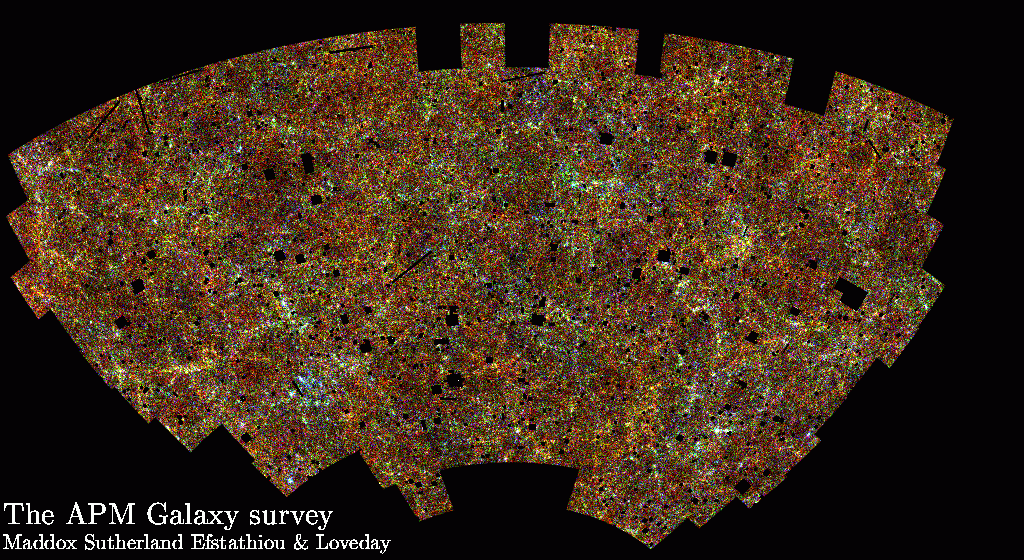
\includegraphics[width=0.6\textwidth]{immagini/APM.png}
    \caption{La giura mostra la distribuzione di ammassi di Galassie nel cielo osservabile, si nota come la distribuzioe risulta pressoché uniforme.}\label{fig:APM}
\end{figure}
\subsection{Espansione dell'universo e Red-Shift}\label{sec:espansione}

Nel 1929 Edwin Hubble si rese conto che le linee spettrali delle galassie venivano spostate verso il rosso proporzionalmente alla loro distanza da noi, ne dedusse che questa variazione cromatica fosse dovuta all'effetto Doppler e che quindi le galassie si stessero allontanando con una certa velocità dall'osservatore. Le galassie sembrano quindi recedere con una velocità proporzionale con la loro distanza.

\begin{figure}
    \centering
    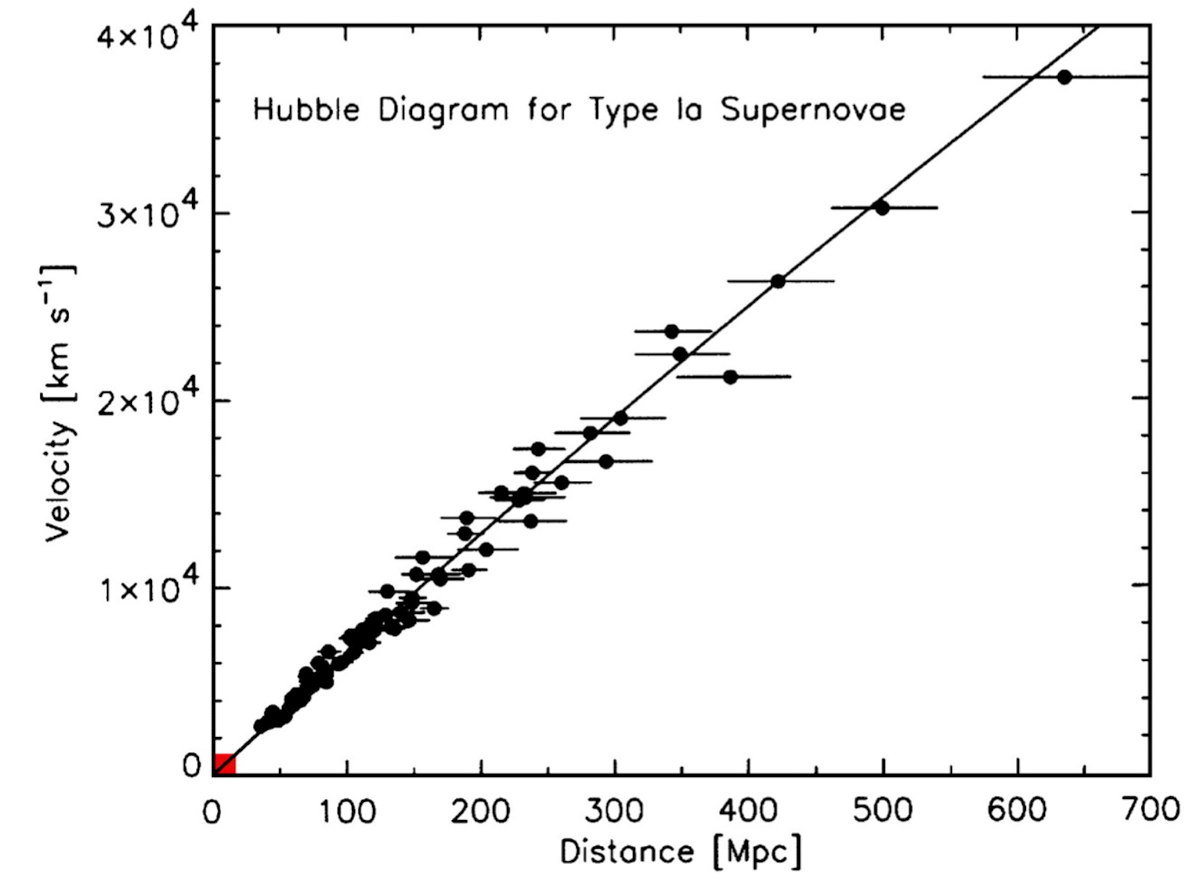
\includegraphics[width=0.5\textwidth]{immagini/redshift.png}
    \caption{La mostra la relazione tra velocità di allontanamento in funzione della distanza, questa è stata stimata misurando la luminosità di supernove di tipo I.a.}\label{fig:redshift}
\end{figure}

Secondo i principi cosmologici l'osservatore non occupa un posto privilegiato nell'Universo, per cui le galassie devono allontanarsi l'una dall'altra, con velocità proporzionale alla distanza tra di loro. Questa dipendenza è ben rappresentata dalla relazione di Hubble, nell equazione~\ref{eq:hubble}
\begin{equation}\label{eq:hubble}
    v = H_0 D
\end{equation}
dove $H_0 \simeq \SI{73}{km.s^{-1}.Mpc^{-1}}$ ($[s^{-1}]$)è la costante di Hubble odierna. Il valore esatto di questa costante è ancora dibattuto soprattutto perché è complesso determinare le distanze esatte tra le varie galassie e distinguere la velocità degli ammassi, rispetto alle velocità delle galassie interne all'ammasso.

Se, quindi, le galassie si stanno allontanando l'una dall'altra senza che esista un centro dell'espansione allora vuol dire che ad espandersi è lo spazio-tempo stesso, il quale trascina con se tutto ciò che contiene. Questa è perciò la causa del \textit{red-shift} che osservava Hubble, infatti se è l'Universo stesso che sis ta espandendo allora la radiazione che lo attraversa si espande insieme a lui e per cui quando arriva ad un osservatore molto distante, sembra spostata verso il rosso. Indichiamo con $z$ il redshift cosmologico e lo calcoliamo con l'equazione~\ref{eq:redshift}
\begin{equation}\label{eq:redshift}
    z = \frac{\lambda_{obs} - \lambda_{em}}{\lambda_{em}}
\end{equation}
dove $\lambda_{em}$ è la unghezza d'onda emessa, mentre $\lambda_{obs}$ è la lunghezza d'onda osservata e modificata rispetto alla $\lambda_{em}$ a causa del redshift.

Mettendo insieme l'equazione~\ref{eq:hubble} di Hubble e l'equazione~\ref{eq:redshift} si ottiene una equivalenza tra redshift e distanza, sappiamo infatti che:
\[
    \frac{\lambda_{obs} - \lambda_{em}}{\lambda_{em}} = \frac{v}{c}
\]
dove $c$ è la velocità della luce e $v$ è la velocità di espansione dell'universo, per cui il redshift $z$ non è altro che il la velocità di espansione dell'universo in unità di velocità della luce.
\[
    v = \frac{\lambda_{obs} - \lambda_{em}}{\lambda_{em}} c
\]
Per cui inserendo ora la relazione di Hubble:
\[
    v = H_0 D = c z
\]
\begin{equation}\label{eq:ditanza-redshift}
    D = \frac{c}{H_0}z
\end{equation}

Si noti che non esistono delle condizioni sul valore che $z$ può assumere, si deduce che potenzialmente può assumere anche valori superiori ad uno, ma questo vorrebbe dire che l'espansione dello spazio-tempo sia più veloce della luce. Questo non è un problema poiché la relatività ristretta impone la velocità della luce come limite all'interno di quello che è il nostro universo, ma non da indicazioni su cosa succeda all'universo stesso al suo esterno.